\documentclass[12pt]{article}

\usepackage{graphicx}
\usepackage[margin=1.0in]{geometry}
\usepackage{amsmath}
\usepackage{cases}
\usepackage{amsfonts}
\usepackage{amssymb}
\usepackage{grffile}
\usepackage{setspace}
\usepackage{listings}

\setlength\parindent{0pt}

\author{Xiaohui Chen \\EID: xc2388}
\title{PHY 362K Homework 6}

\begin{document}
\maketitle

\begin{spacing}{2.0}

\section{} %1

\subsection*{(a)}

\begin{figure}
  \centering
  % Requires \usepackage{graphicx}
  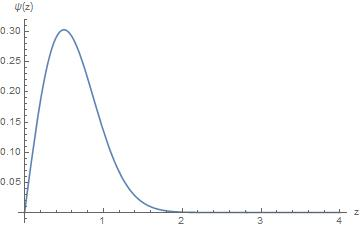
\includegraphics[width=5in]{out1}\\
  \caption{Plot of $\psi(z)$}\label{out1}
\end{figure}


The wave function is shown in Figure \ref{out1}. From Figure \ref{out1}. We can see that the wave function approaches $0$ at both $z=0$ and at infinity. Also, it has a local maximum value, which indicates the object getting to the highest point. Therefore this wave function is a suitable approximation

The wave function is $\psi(z)= Aze^{-\alpha z^2}$

Since the wave function is normalized, we get that $\int_{0}^{\infty} |\psi(z)|^2 dz = A^2 \int_{0}^{\infty} z^2e^{-2\alpha z^2} dz=1$

Use Mathematica, $A^2 \int_{0}^{\infty} z^2 e^{-2*\alpha z^2} dz= \frac{\sqrt{\frac{\pi }{2}} A^2}{8 \alpha ^{3/2}} = 1$

$\therefore A=2\left(\frac{2\alpha}{\pi}\right)^{\frac{3}{4}}$

Therefore the wave function is $\psi(z)= 4\left(\frac{2\alpha}{\pi}\right)^{\frac{3}{2}} ze^{-\alpha z^2}$

$\langle H \rangle= \langle T \rangle + \langle V \rangle$

$\langle T \rangle= -\frac{\hbar^2}{2m} 4\left(\frac{2\alpha}{\pi}\right)^{\frac{3}{2}} \int_{0}^{\infty} ze^{-\alpha z^2} \frac{d^2 ze^{-\alpha z^2}}{d z^2} dz = \frac{3 \alpha  \hbar ^2}{2 m}$ (using Mathematica)

$\langle V \rangle= 4mg\left(\frac{2\alpha}{\pi}\right)^{\frac{3}{2}} \int_{0}^{\infty} z^3 e^{-2\alpha z^2} dz = mg\sqrt{\frac{2}{\pi \alpha}}$ (using Mathematica)

$\therefore \langle H \rangle= \frac{3 \alpha  \hbar ^2}{2 m} + mg\sqrt{\frac{2}{\pi \alpha}}$

$\frac{d}{dz} \langle H \rangle = \frac{3 \hbar ^2}{2 m}-\frac{g m}{\sqrt{2 \pi } \alpha ^{3/2}}$

In order to get the minimum value of $\langle H \rangle$, we have to let $\frac{d}{dz} \langle H \rangle=0$. Therefore $\alpha = \frac{\sqrt[3]{\frac{2}{\pi }}}{3^{2/3} \left(\frac{\hbar ^2}{g m^2}\right)^{2/3}}$

Plug in the value of $\alpha$ and we get $E_{gs} \approx \langle H \rangle_{min} = \sqrt[3]{\frac{81mg^2\hbar^2}{4\pi}}$

The Mathematica code used in this part is shown below:

\begin{lstlisting}[language=Mathematica,breaklines=true,frame=single]
Simplify[Integrate[
  A^2*z^2*Exp[-2*\[Alpha]*z^2], {z, 0,
   Infinity}], \[Alpha] \[Element] Reals && \[Alpha] > 0]

Simplify[Solve[(A^2 Sqrt[\[Pi]/2])/(8 \[Alpha]^(3/2)) == 1, A], A \[Element] Reals && A > 0]

A := (2 2^(3/4) \[Alpha]^(3/4))/\[Pi]^(1/4)
\[Psi][z_] := A*z*Exp[-\[Alpha]*z^2]

Simplify[-(\[HBar]^2/(2*m))*
  Integrate[\[Psi][z]*D[\[Psi][z], {z, 2}], {z, 0,
    Infinity}], \[Alpha] \[Element] Reals && \[Alpha] > 0]

T[\[Alpha]_] := (3 \[Alpha] \[HBar]^2)/(2 m)

Simplify[m*g*
  Integrate[
   z*\[Psi][z]*\[Psi][z], {z, 0, Infinity}], \[Alpha] \[Element]
   Reals && \[Alpha] > 0]

V[\[Alpha]_] := (g m Sqrt[2/\[Pi]])/Sqrt[\[Alpha]]
H[\[Alpha]_] := T[\[Alpha]] + V[\[Alpha]]
D[H[\[Alpha]], {\[Alpha], 1}]

Simplify[Solve[-((g m)/(Sqrt[2 \[Pi]] \[Alpha]^(3/2))) + (3 \[HBar]^2)/(2 m) == 0, \[Alpha]], \[Alpha] >
   0 && \[Alpha] \[Element] Reals]

H[(2/\[Pi])^(1/3)/(3^(2/3) (\[HBar]^2/(g m^2))^(2/3))]
\end{lstlisting}

\subsection*{(b)}

In classical region, $E > V(x)$

At the turning point, $E=V(x)$. Therefore the turning point is $a=\frac{E}{mg}$

Let $p(z)= \sqrt{2m(E-mgz)}$

In classical region, we have $\psi_1(z)= \frac{C}{\sqrt{p}} \left[ \sin \phi(z) + \cos \phi(z) \right]$, where $\phi(z)= \frac{1}{\hbar} \int_{0}^{z} p(z') dz' $

$\because \psi_1(0)=0$

$\therefore \cos \phi(0)=0$

$\psi_1(z)= \frac{C}{\sqrt{p(z)}} \sin \left[\frac{1}{\hbar} \int_{0}^{z} p(z') dz' \right]= \frac{C}{\sqrt{p(z)}} \cos \left[\frac{1}{\hbar} \int_{0}^{z} p(z') dz' - \frac{\pi}{2} \right]$ for $0<z<a$

At the turning point, according to the connection formulas shown in textbook, we have

$\psi_2(z) = \frac{C'}{\sqrt{p(z)}} \sin \left[ \frac{1}{\hbar} \int_z^a p(z') dz' + \frac{\pi}{4} \right]= \frac{C'}{\sqrt{p(z)}} \cos \left[ \frac{1}{\hbar} \int_z^a p(z') dz' - \frac{\pi}{4} \right]$ for $0<z<a$

Since we need $\psi_1(z)=\psi_1(z)$, we have

$\frac{1}{\hbar} \int_{0}^{z} p(z') dz' - \frac{\pi}{2} \frac{1}{\hbar} \int_z^a p(z') dz' - \frac{\pi}{4} = n\pi$

$\therefore \frac{1}{\hbar} \int_{0}^{a} p(z) dz= (n+ \frac{3}{4})\pi$

$\int_{0}^{a} \sqrt{2m(E-mgz)} dz= (n+ \frac{3}{4})\hbar \pi$

Use Mathematica, we therefore find

$E=\frac{1}{3} \sqrt[3]{9\pi^2 \hbar^2 g^2 m} \left( n+\frac{3}{4} \right)^{2/3}$

The Mathematica code used in this part is shown below:

\begin{lstlisting}[language=Mathematica,breaklines=true,frame=single]
Solve[Integrate[
   Sqrt[2*m*(En - m*g*z)], {z, 0,
    En/(m*g)}] == (n + 3/4)*\[HBar]*\[Pi], En]
\end{lstlisting}

\subsection*{(c)}

The time independent Schrodinger equation is

$-\frac{\hbar^2}{2m} \frac{d^2 \psi}{d z^2} + V(x)\psi = E \psi $

The Schrodinger equation in this question is therefore

$-\frac{\hbar^2}{2m} \frac{d^2 \psi}{d z^2} + mgz \psi = E \psi$

$\because x=\frac{z}{b}$

$\therefore dz^2 = b^2 dx^2$

The Schrodinger equation becomes $-\frac{\hbar^2}{2m} \frac{d^2 \psi}{d x^2} +  b^2 mgz \psi = b^2 E \psi$

This is equivalent to $-\frac{1}{2} \frac{d^2 \psi}{d x^2} +  \frac{m^2 g b^3}{\hbar^2} x\psi = \frac{m b^2}{\hbar^2} E \psi$

$\because b=\left( \frac{\hbar^2}{m^2 g} \right)^{1/3}$

$-\frac{1}{2} \frac{d^2 \psi}{d x^2} +  \frac{m^2 g }{\hbar^2} \frac{\hbar^2}{m^2 g} x\psi = \frac{m b^2}{\hbar^2} E \psi$

$\therefore -\frac{1}{2} \frac{d^2 \psi}{d x^2} + x\psi = \epsilon E \psi$, where $\epsilon = \frac{E}{\hbar^2/mb^2}$

\subsection*{(d)}

%We use the following Mathematica code to determine the ideal values of $\epsilon$:
%
%\begin{lstlisting}[language=Mathematica,breaklines=true,frame=single]
%pfun = ParametricNDSolveValue[{-(1/2)*\[Psi]''[x] +
%     x*\[Psi][x] == \[Epsilon]*\[Psi][x], \[Psi][0] == 0, \[Psi]'[0] ==
%     1}, \[Psi], {x, 0, 6}, \[Epsilon]]
%Plot[pfun[\[Epsilon]][6], {\[Epsilon], 1, 7}]
%
%\end{lstlisting}
%
%\begin{figure}
%  \centering
%  % Requires \usepackage{graphicx}
%  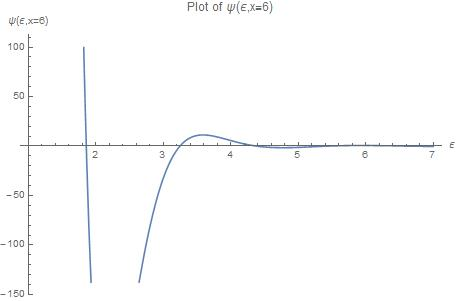
\includegraphics[width=5in]{out2}\\
%  \caption{Parametric Function $\psi(\epsilon,x)$ when $x=6$ and $\epsilon$ varies}\label{out2}
%\end{figure}
%
%
%The plot of the function $\psi(\epsilon,x=6)$ is shown in  is shown in Figure \ref{out2}. Since we are solving this parametric differential equation from 0 to 6. Ideally we want $\psi(x=6)=0$. Therefore we can find the values of $\epsilon$ such that $\psi(\epsilon,x=6)=0$


\begin{figure}
  \centering
  % Requires \usepackage{graphicx}
  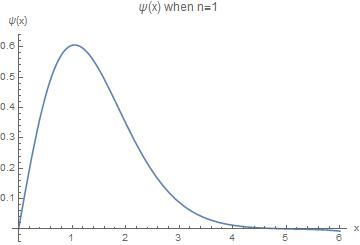
\includegraphics[width=5in]{out3}\\
  \caption{Plot of $\psi(x)$ when $n=1$ }\label{out3}
\end{figure}

When $\epsilon \approx 1.85576$, $n=1$, the plot is shown in Figure \ref{out3}. In this case, $E=1.85576 \frac{\hbar^2}{mb^2} = 1.85576 \sqrt[3]{mg^2 \hbar^2}$

\begin{figure}
  \centering
  % Requires \usepackage{graphicx}
  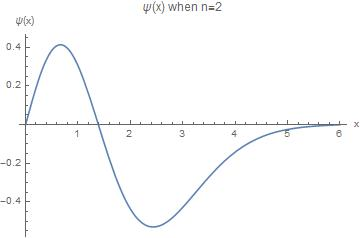
\includegraphics[width=5in]{out4}\\
  \caption{Plot of $\psi(x)$ when $n=2$ }\label{out4}
\end{figure}

When $\epsilon \approx 3.24464$, $n=2$, the plot is shown in Figure \ref{out4}. In this case, $E= 3.24464 \sqrt[3]{mg^2 \hbar^2}$

\begin{figure}
  \centering
  % Requires \usepackage{graphicx}
  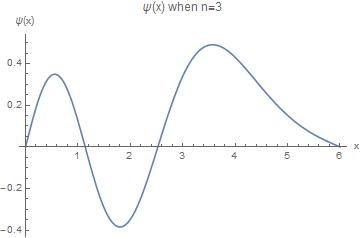
\includegraphics[width=5in]{out5}\\
  \caption{Plot of $\psi(x)$ when $n=3$ }\label{out5}
\end{figure}

When $\epsilon \approx 4.38491$, $n=3$, the plot is shown in Figure \ref{out5}. In this case, $E= 4.38491 \sqrt[3]{mg^2 \hbar^2}$

\begin{figure}
  \centering
  % Requires \usepackage{graphicx}
  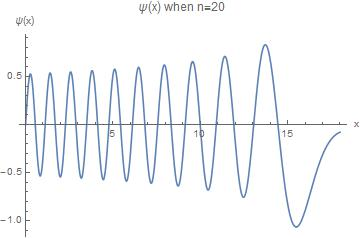
\includegraphics[width=5in]{out6}\\
  \caption{Plot of $\psi(x)$ when $n=20$ }\label{out5}
\end{figure}

When $\epsilon \approx 16.29999$, $n=20$, the plot is shown in Figure \ref{out5}. In this case, $E= 16.29999 \sqrt[3]{mg^2 \hbar^2}$

The Mathematica code used in this part is shown below:

\begin{lstlisting}[language=Mathematica,breaklines=true,frame=single]
Clear[\[Epsilon], \[Psi]]
pfun = ParametricNDSolveValue[{-(1/2)*\[Psi]''[x] +
     x*\[Psi][x] == \[Epsilon]*\[Psi][x], \[Psi][0] ==
    0, \[Psi]'[0] == 3}, \[Psi], {x, 0, 20}, \[Epsilon]]
    
Plot[pfun[1.85576][x], {x, 0, 6}, PlotLabel -> "\[Psi](x) when n=1",
 AxesLabel -> {"x", "\[Psi](x)"}]
 
Plot[pfun[3.24464][x], {x, 0, 6}, PlotLabel -> "\[Psi](x) when n=2",
 AxesLabel -> {"x", "\[Psi](x)"}]
 
Plot[pfun[4.38491][x], {x, 0, 6}, PlotLabel -> "\[Psi](x) when n=3",
 AxesLabel -> {"x", "\[Psi](x)"}]

Plot[pfun[16.29999][x], {x, 0, 18},
 PlotLabel -> "\[Psi](x) when n=20", AxesLabel -> {"x", "\[Psi](x)"}]
\end{lstlisting}

\subsection*{(e)}

\begin{tabular}{|c|c|c|c|c|c|}
  \hline
  % after \\: \hline or \cline{col1-col2} \cline{col3-col4} ...
   & Numerical & WKB & Variational & WKB Error \% & Variational Error \%\\
   \hline
  $n=1$ & $1.85576 \sqrt[3]{mg^2 \hbar^2}$ & $0.48407 \sqrt[3]{9\pi^2 \hbar^2 g^2 m}$ & $\sqrt[3]{\frac{81mg^2\hbar^2}{4\pi}}$ & $16.3859 \%$ & $0.2851 \%$\\
  \hline
  $n=2$ & $3.24464 \sqrt[3]{mg^2 \hbar^2}$ & $0.65429\sqrt[3]{9\pi^2 \hbar^2 g^2 m}$ & N/A & $10.0258 \%$ & N/A \\
  \hline
  $n=3$ & $4.38491 \sqrt[3]{mg^2 \hbar^2}$ & $0.80457\sqrt[3]{9\pi^2 \hbar^2 g^2 m}$ & N/A & $18.1314 \%$ &N/A \\
  \hline
  $n=20$ & $16.29999 \sqrt[3]{mg^2 \hbar^2}$ & $2.51704\sqrt[3]{9\pi^2 \hbar^2 g^2 m}$ & N/A & $31.1003 \%$ &N/A \\
  \hline
\end{tabular}

\section{} %2

\subsection*{(a)}

We let $|\psi_{gs}\rangle = |\psi_1 \rangle$

Then $\langle \psi|\psi_1 \rangle = 0$

Since we know that $\psi= \sum\limits_{n=1}^{\infty} C_n \psi_n$, $\langle \psi| \psi_1 \rangle= \sum\limits_{n=1}^{\infty} C_n \langle \psi_n | \psi_1 \rangle = \sum\limits_{n=1}^{\infty} C_n \delta_{n1}$

$\because \langle \psi|\psi_1 \rangle = 0$

$\therefore C_1=0$

We also know that $\langle H \rangle = \langle \psi|H|\psi \rangle = \sum\limits_{n=1}^{\infty} |C_n|^2 E_n$

$\because C_1=0$

$\therefore \langle H \rangle= \sum\limits_{n=2}^{\infty} |C_n|^2 E_n$

Since the excited state energies are larger than the ground state energies, $\langle H \rangle \ge \sum\limits_{n=2}^{\infty} |C_n|^2 E_{gs}$

$\sum\limits_{n=2}^{\infty} |C_n|^2 \le 1$

$\therefore \langle H \rangle \ge E_{gs}$

\subsection*{(b)}

We know that $\int_{-\infty}^{\infty} |\psi(x)|^2 =1$

Using Mathematica, we get that $\int_{-\infty}^{\infty} A^2x^2e^{-2bx^2} = \frac{\sqrt{\frac{\pi }{2}} A^2}{4 b^{3/2}}$

$\therefore A^2= 4b\sqrt{\frac{2b}{\pi}}$

As for the harmonic oscillator, $H= -\frac{\hbar^2}{2m} \frac{d}{dx^2}+ \frac{1}{2} m\omega^2 x^2$

$\langle T \rangle = -\frac{\hbar^2}{2m} \int_{-\infty}^{\infty} \psi^{*}(x) \frac{d^2\psi(x)}{dx^2} dx = \frac{3 b \hbar ^2}{2 m}$

$\langle V \rangle= \frac{1}{2}m\omega^2 \int_{-\infty}^{\infty} \psi^{*}(x)x^2\psi(x) dx = \frac{3 m \omega ^2}{8 b}$

$\therefore \langle H \rangle = \langle T \rangle + \langle V \rangle= \frac{3 m \omega ^2}{8 b}+\frac{3 b \hbar ^2}{2 m}$

$\frac{d\langle H \rangle}{db}= \frac{3 \hbar ^2}{2 m}-\frac{3 m \omega ^2}{8 b^2}$

In order to find the minimum value, we have to let $\frac{d\langle H \rangle}{db}= 0 $

Therefore, $b=\frac{m \omega }{2 \hbar }$

Plug in the value of $b$, we get that $\langle H \rangle_{min}= \frac{3 \omega  \hbar }{2}$

The exact value of the first excited state is $E_1= \frac{3}{2} \hbar \omega$. Theretofore, $\langle H \rangle_{min}= E_1$

The Mathematica code used in this part is shown below:

\begin{lstlisting}[language=Mathematica,breaklines=true,frame=single]
Clear[\[Psi], A, b]
\[Psi][x_] := A*x*Exp[-b*x^2]
Simplify[Integrate[Abs[\[Psi][x]]^2, {x, -Infinity, Infinity}],
 A \[Element] Reals && b \[Element] Reals && A > 0 && b > 0]
 
Solve[(A^2 Sqrt[\[Pi]/2])/(4 b^(3/2)) == 1, A]

T[x_] := -(\[HBar]^2/(2*m))*
  Integrate[\[Psi][x]*D[\[Psi][x], {x, 2}], {x, -Infinity, Infinity}]
V[x_] := (1/2)*m*\[Omega]^2*
  Integrate[x^2*\[Psi][x]*\[Psi][x], {x, -Infinity, Infinity}]
En[x_] := T[x] + V[x]

D[En[x], {b, 1}]

Solve[-((3 m \[Omega]^2)/(8 b^2)) + (3 \[HBar]^2)/(2 m) == 0, b]

b := (m \[Omega])/(2 \[HBar])
En[x]
\end{lstlisting}

\section{} %3

\subsection*{(a)}

We know that the probability of tunneling is $T\approx e^{-2\gamma}$

Here $\gamma \equiv \frac{1}{\hbar} \int_{0}^{a} |p(x)| dx$ and $p(x)= \sqrt{2m(V_0-e\mathcal{E}x-E)}= \sqrt{2m(W-e\mathcal{E}x)}$

The end point $a$ is given by $W=e\mathcal{E}a$

$\therefore a=\frac{W}{e\mathcal{E}}$

In this case, $\gamma= \frac{1}{\hbar} \int_{0}^{\frac{W}{e\mathcal{E}}} \sqrt{2m(W-e\mathcal{E}x)} dx = \frac{2 \sqrt{2} W \sqrt{m W}}{3 e \mathcal{E} \hbar}$

$\therefore T(\mathcal{E})= e^{-\mathcal{E}_0/\mathcal{E}}$, where $\mathcal{E}_0 = \frac{4}{3}\frac{\sqrt{2m}}{\hbar} \frac{W^{3/2}}{e}$

The Mathematica code used in this part is shown below:

\begin{lstlisting}[language=Mathematica,breaklines=true,frame=single]
\[Gamma] :=
 1/\[HBar]*
  Integrate[
   Sqrt[2 m*(W - e*\[CapitalEpsilon]*x)], {x, 0,
    W/(e*\[CapitalEpsilon])}]
\end{lstlisting}

\subsection*{(b)}

The mass of electron is $m=9.10938291*10^{-31} kg$

Using Mathematica, we can get $\mathcal{E}_0 = 6.62971*10^{10}$

Since $\frac{\mathcal{E}_0}{\mathcal{E}}= 50$, we get that $\mathcal{E}= \frac{\mathcal{E}_0}{50} = 1.32594*10^{9} V\cdot m^{-1}$

\subsection*{(c)}

From part (a) we know that the endpoint $a$ is given by $a=\frac{W}{e\mathcal{E}}$ 

$\therefore L =\frac{4.55*1.6*10^{-19}}{1.6*10^{-19}*1.32594*10^{9}} m= 3.4315*10^{-9} m$

\end{spacing}
\end{document} 